\documentclass[a4paper,14pt]{article}
\usepackage{lscape}
%%% Страница
\usepackage{extsizes} % Возможность сделать 14-й шрифт
\usepackage{geometry} % Простой способ задавать поля
        \geometry{top=25mm}
        \geometry{bottom=30mm}
        \geometry{left=30mm}
        \geometry{right=20mm}
 %
% https://ctan.math.illinois.edu/macros/latex/contrib/enumitem/enumitem.pdf
%\usepackage{enumitem}

\usepackage[T1,T2A]{fontenc}
\usepackage[utf8]{inputenc}
\usepackage{amssymb,amsmath}
\usepackage{float}
\usepackage[unicode, pdftex]{hyperref}
\usepackage[europeanresistors,americaninductors]{circuitikz}
\usetikzlibrary{calc}
\usepackage[T1,T2A]{fontenc}
\usepackage[utf8]{inputenc}


\usepackage{amssymb,amsmath}
\usepackage{float}
\usepackage[unicode, pdftex]{hyperref}

\usepackage[inline]{enumitem}
%\usepackage{cleveref}
%\crefname{subsectioni}{enumi}{examples}
%\renewcommand{\labelenumi}{\thesubsection.\arabic{enumi}}
%https://tex.stackexchange.com/questions/466153/cross-referencing-multiple-items

\usepackage{tikz}
\usepackage{rotating}
%\usepackage[landscape]{geometry}
\usepackage{graphicx}
\graphicspath{{pictures/}}
\DeclareGraphicsExtensions{.pdf,.png,.jpg}
\usepackage{pgfplots}
\usepackage{wrapfig}
\usepackage{rotating}
\usepackage{lipsum}
\usepackage{nccmath}
\usepackage{caption}
\usepackage{siunitx}
%\usepackage[american,cuteinductors,smartlabels]{circuitikz}
%\usepackage[backend=biber]{biblatex}

\usepackage[]{hyperref}
\ctikzset{bipoles/thickness=1}
\ctikzset{bipoles/length=0.8cm}
\ctikzset{bipoles/diode/height=.375}
\ctikzset{bipoles/diode/width=.3}
\ctikzset{tripoles/thyristor/height=.8}
%\ctikzset{tripoles/thyristor/width=1}
\ctikzset{tripoles/thyristor/width=0.8}
\ctikzset{bipoles/vsourceam/height/.initial=.7}
\ctikzset{bipoles/vsourceam/width/.initial=.7}

\tikzstyle{every node}=[font=\small]
\tikzstyle{every path}=[line width=0.8pt,line cap=round,line join=round]

\ctikzset{resistor = european}
\ctikzset{inductor = american}
\ctikzset{tripoles/thyristor/height=0.55}

\ctikzset{bipoles/cuteindictor/coils/.initial=3}
\ctikzset{bipoles/americanindictor/coils/.initial=3}
\ctikzset{bipoles/cuteindictor/coils/.initial=3}
\ctikzset{bipoles/americanindictor/coils/.initial=3}
\hypersetup{
colorlinks=false,
}
\usepackage{textcomp}

\begin{document}


 

\section{Research of 3-phase half-wave thyristor converters}

The aim of the work is an experimental study of thyristor converters which made according to schemes with zero tap of the secondary windings of the transformer.

\subsection{Lab Description}

At the laboratory bench, you can examine the following converter circuits:

\begin{itemize}
\item 3-phase half-wave non-reversible (Fig. 5.1, a);

\item 6-phase according to the connection diagram of the transformer windings "6-phase star with zero tap" (Fig. 5.1, 6);

\item 6-phase according to the connection scheme of the transformer windings 
"star -- two reverse stars with equalization reactor" (Fig. 5-1, c);

\item 3-phase half-wave reverse according to the cross-section diagram, with joint coordinated control (Fig. 5.1, d).
\end{itemize}

To build any of these circuits, one or two 3-phase a half-wave thyristor groups (V1-VЗ, V4-V6) are used, which are powered from a 3-phase 3-winding transformer $T$ (Fig. 5.2).

The secondary windings $T$ are connected according to the "two reverse stars" circuit, which provides a phase shift of the voltages between them by 180 electrical degrees.

In fig. 5.2 shows a diagram of the power part of the laboratory bench, and in fig. 5.3 is a diagram of the control circuits.

The laboratory stand is switched on by switch $Q1$, and the preparation of the inclusion of the corresponding variant of the converter circuit is made by contactors $K1$, $K2$ and switches $QЗ$, $Q4$.

To turn on the 3-phase half-wave circuit (Fig. 5.1, a), it is necessary, not including the contactors, to turn on the switches $QЗ$, $Q4$.
To ensure the inclusion of a 6-phase half-bridge converter circuit (Fig. 5.1, 6), it is additionally necessary to turn on the contactor $K1$ by pressing the $SB2$ button (Fig. 5.3).
To prepare the inclusion of the circuit in Fig. 5.1, turn off $Q3$, turn on $Q4$ and $K1$.
To enable the reverse circuit of the converter, first turn on $Q3$, turn off $Q4$ and $K1$ (using the $SB1$ button) and turn on $K2$ (using the $SBЗ$ button).

The load of the converter can be either an active resistance (resistor $R4$) or an armature of a direct current machine $M1$ with a smoothing choke $L4$ connected in series.
Disconnecting $K4$ and connecting $M1$ is done by contactor $K3$ by pressing the $SB4$ button.
To control the armature current $M1$, when the motor $M2$ is mounted on the shaft $M1$ and connected via the $Q5$ switch to the 380/220V network, the potentiometer $RP2$ must change the current in the field winding $M1.2$.

3-phase thyristor groups are controlled from two pulse-phase control systems SPPC1 and SPPC2.

When non-reversible 6-pulse converter circuits are switched on (Fig. 5.1, 6, c), the inputs of two 3-phase SPPCs are connected by the $K2$ block contacts in parallel, which is equivalent to combining them into one 6-phase SPPC.
When the reverse converter circuit is switched on, the inputs of the 3-phase SPPCs are connected by the $K2$ block contacts in the opposite direction, which allows for joint coordinated control of the thyristor groups.

The schemes used in the SPPC laboratory setup is the same as in the scheme described in 3.
Potentiometers $R15-R17$ of input SPPC nodes (see. Fig. 3.1), designed to adjust the initial, minimum and maximum values of the angle of regulation, are placed on the front panel of the laboratory bench.
This allows you to configure the phase characteristics of SPPC to control both reversible and non-reversible versions of converter circuits.

The following measuring instruments are installed on the front panel of the laboratory bench:

\begin{itemize}
\item ammeter $P7$ and voltmeter $P6$, designed to measure the current and voltage of one phase of the primary winding of the transformer $T$;

\item measuring set $P8$, which allows measuring active ($P$) and reactive ($Q$) power, as well as currents and voltages on the primary side of the transformer transformer $T$;

\item ammeter $P10$ and voltmeter $P9$, designed to measure rectified current and voltage;

\item voltmeter $P1$, measuring the control voltage at the input of SPPC;

\item a voltmeter $P2$, designed to measure the phase voltage of the valve coil;

\item ammeters $P4$ and $P11$, measuring currents at the output of 3-phase converter groups $V1-V3$ and $V4-V6$;

\item ammeter $P5$, which serves to indicate the current in the field winding $M1.2$ of the DC machine $M$1;

\item ammeter $РЗ$, used to indicate the current in the neutral wire of the primary winding of the transformer $T$.
\end{itemize}

An electronic oscilloscope is used to measure the angle of regulation of the converters and to observe the voltage and current curves of individual sections of the converter circuit (terminals $X1-X10$).

\subsection{Task: Research of non-reversible thyristor converters}

\begin{enumerate}[label=\emph{\arabic*}. , ref=\emph{\thesubsection.\arabic*}, leftmargin=0pt, labelindent=\parindent]
\item\label{taskI:itm1}For each of the options for power circuits of non-reversible thyristor converters specified by the teacher, set the following values of the minimum, initial and maximum control angles using regulating potentiometers of the input SPPC nodes:
$\alpha_{min} = 0^\circ$, $\alpha_{initial}= 90^\circ$, $\alpha_{max} = 145^\circ$.

\item\label{taskI:itm2} observe and plot the control characteristic of SPPC $\alpha = f(U_{ctrl})$.

\item\label{taskI:itm3}  For the converter circuits studied in \ref{taskI:itm1}, when operating under active load, observe and plot the control characteristics of the converters $U_d = f (\alpha)$, $U_d = f (U_{ctrl})$, 
draw the rectified voltage curves $u_d = f(\omega t)$ from the oscilloscope screen (terminals $X6$, $X8$) at control angles of 15, 75 and $105^\circ$.

\item\label{taskI:itm4} For the same converter circuits when working on the anchor of an electric DC machine in rectifier and inverter modes, it is necessary to plot graphs:

\begin{itemize}
\item regulating characteristics $U_d = f (\alpha)$, $U_d = f (U_{ctrl})$ and 
the dependence $\alpha = f (U_{ctrl})$ during operation of the converters to the anchor of an electric DC machine 
in both rectifier and inverter modes with a constant value of the rectified current $I_d = 1A$ ;

\item a family of external characteristics with the values of the angle of regulation of 15, 75, 105 and $120^\circ$;

\item energy characteristics of the converters -- the dependence of efficiency ($\eta$), 
reactive power ($Q$) and power factor ($\lambda$) on the rectified voltage at a constant value of the rectified current 
$I_d = 4A$.
\end{itemize}

\item\label{taskI:itm5} For the converter circuits studied in \ref{taskI:itm4} 
and the indicated values of the angle $\alpha$, draw the rectified voltage curves 
$u_d = f (\omega t)$ (terminals $X6$, $X8$) with the rectified current $I_d = 2A$ from the oscilloscope screen.
\end{enumerate}


\subsection{Task: Research reverse thyristor converter}

\begin{enumerate}[label=\emph{\arabic*}. , ref=\emph{\thesubsection.\arabic*}, leftmargin=0pt, labelindent=\parindent]

\item \label{taskII:itm1}For a 3-phase half-wave reversal converter circuit, use the regulating potentiometers of the input nodes SPPC 1 and SPPC 2 to set the following values of the control angles: $\alpha_{min1} = \alpha_{min2} =  35^\circ$,
$\alpha_{initial} = 90^\circ$, $\alpha_{max1} = \alpha_{max2} = 145^\circ$.

\item\label{taskII:itm2} Observe and plot on one graph the regulating characteristics of SPPC 1 and SPPC 2 $\alpha_1= f (U_{ctrl})$ 
and $\alpha_2 = f (U_{ctrl})$.

\item\label{taskII:itm3} During operation of the converter to the anchor of the DC machine, observe and plot on one graph 
the regulating characteristics $U_d = f (U_{ctrl})$ and the dependence of the surgei(equalizing) current 
on the control voltage $Iу = f (Uу)$ at $Id = \pm 2A$.

\item\label{taskII:itm4} When working on an anchor of a DC machine, observe and plot a family of external characteristics of the converter 
for both directions of the rectified current at control voltages $U_{ctrl}$ corresponding to the following values 
of the control angle $\alpha_1$:  35, 75, 105, and $145^\circ$.


\item\label{taskII:itm5} Draw the rectified voltage curves of the converter 
$u_d = f (\omega t)$ (terminals $X6$, $X8$), $u_{d2} = f (\omega t)$ (terminals $X3$, $X8$) from the oscilloscope screen.
\end{enumerate}

\subsection{Methodological instructions how to perform the tasks}

\begin{enumerate}[label=\emph{\arabic*}. , ref=\emph{\thesubsection.\arabic*}, leftmargin=0pt, labelindent=\parindent]
\item The values $\alpha_{min}, \alpha_{initial}, \alpha_{max}$   for each investigated converter circuit 
should be set using an oscilloscope along a curve
$u_d = f (\omega t)$ when operating the converter to the anchor of a DC machine at $I_d \approx 2 A$.
Setting the sweep of the oscilloscope must be done so that the entire range of changes in 
the angle of regulation fits on the screen. 
The angle a should be counted from its zero value according to the sinusoid of one of the phases of the converter.

\item Voltmeters $P1$, $P9$, potentiometer $RP1$ and an oscilloscope are used to take 
the regulating characteristics of SPPC (see \ref{taskI:itm2}; \ref{taskII:itm2}) 
and converters (see \ref{taskI:itm3}; \ref{taskII:itm3}).

\item Before connecting a DC motor to the armature converter $M1.1$ 
(see \ref{taskI:itm4}; \ref{taskII:itm3}--\ref{taskII:itm5}), set the potentiometers $RP1$, $RP2$ to zero values, 
respectively, of the rectified voltage (voltmeter $P9$) and the excitation current in winding $M1.2$ 
(milliammeter $P5$), and turn on $Q5$.

After turning on $K3$ when adjusting the angles $\alpha$, it is necessary to monitor the value of the rectified current 
by the ammeter $P10$, not even allowing it to increase briefly above 6A by changing the current in the winding $M1.2$.

\item When removing the external characteristics of the converters (see \ref{taskI:itm4}; \ref{taskII:itm4}), 
a continuous increase in the rectified current above 4A should not be allowed.

\item To take the energy characteristics of the converters (see \ref{taskI:itm4}; \ref{taskII:itm4}), 
the measuring set $P8$ is used to determine the total power and its active and reactive components on the side 
of the supply network, and devices $P9$, $P10$ on the constant side current.

Efficiency should be determined using expressions:
\begin{itemize}
        \item in rectifier mode ($U_d> 0$):
$$
                \eta = \frac{U_dI_d}{P}
$$
        \item in inverter mode ($U_d <0$):
$$
                \eta = \frac{P}{U_dI_d}
$$

\end{itemize}


The power factor is calculated by the ratio

$$
\lambda = \frac{P}{3I_{P7}U_{P6}}
$$

where $P$ is the active power measured by the set of $P8$; $I_{P7}$, $U_{P6}$ -- phase current and 
voltage values measured by devices $P7$ and $P6$, respectively.

Graphs of energy characteristics are constructed in relative units in the form of dependencies:

$$
                \eta = f(\overline{U_d}; \overline{q}) = f(\overline{U_d}); \lambda = f(\overline{U_d})
$$

where ${\displaystyle Ud = \frac{U_d}{E_{d0}}}$ is the relative value of the rectified voltage,
${\displaystyle q = \frac{Q}{E_{d0}I_d}}$ is the relative value of reactive power; $E_{d0}$
is the maximum value of the rectified EMF of the converter.
The value of $E_{d0}$ is determined based on the readings of $PV1$ from the ratio

$$
E_{d0} = \frac{3\sqrt{2}}{\pi} U_{PV1}
$$


In this case, the absolute value of the reactive power $Q$ is measured by the set $P8$, 
and $Ed0$ is calculated by the expression

$$
E_{d0} = \frac{m}{\pi} \sqrt{2} E_{P2} \sin\frac{\pi}{m}
$$

where $m$ is the number of converter phases equal to 3 for the circuits shown in Fig. 5.1, a, c, d, 
and equal to 6 for the circuit shown in Fig. 5.1, 6; $U_{P2}$ -- voltage measured by the device $P2$ 
at zero value of the rectified current.

\item The value of the equalizing(surge) current $I_{equalizing}$ in the circuit of the reversing converter 
(see \ref{taskII:itm3}) is taken equal to the smaller of the currents of two valve groups, 
determined by ammeters $P4$ and $P11$.

\end{enumerate}

\subsection{Report content}

The report should include:

\begin{enumerate}
\item a diagram of a laboratory setup with a brief description of it and a diagram of the power circuits of the investigated converters;

\item tables, graphs specified in the task of the characteristics of the investigated transducer and waveform;

\item brief conclusions on the results of research.
\end{enumerate}

%\begin{figure}[!ht]
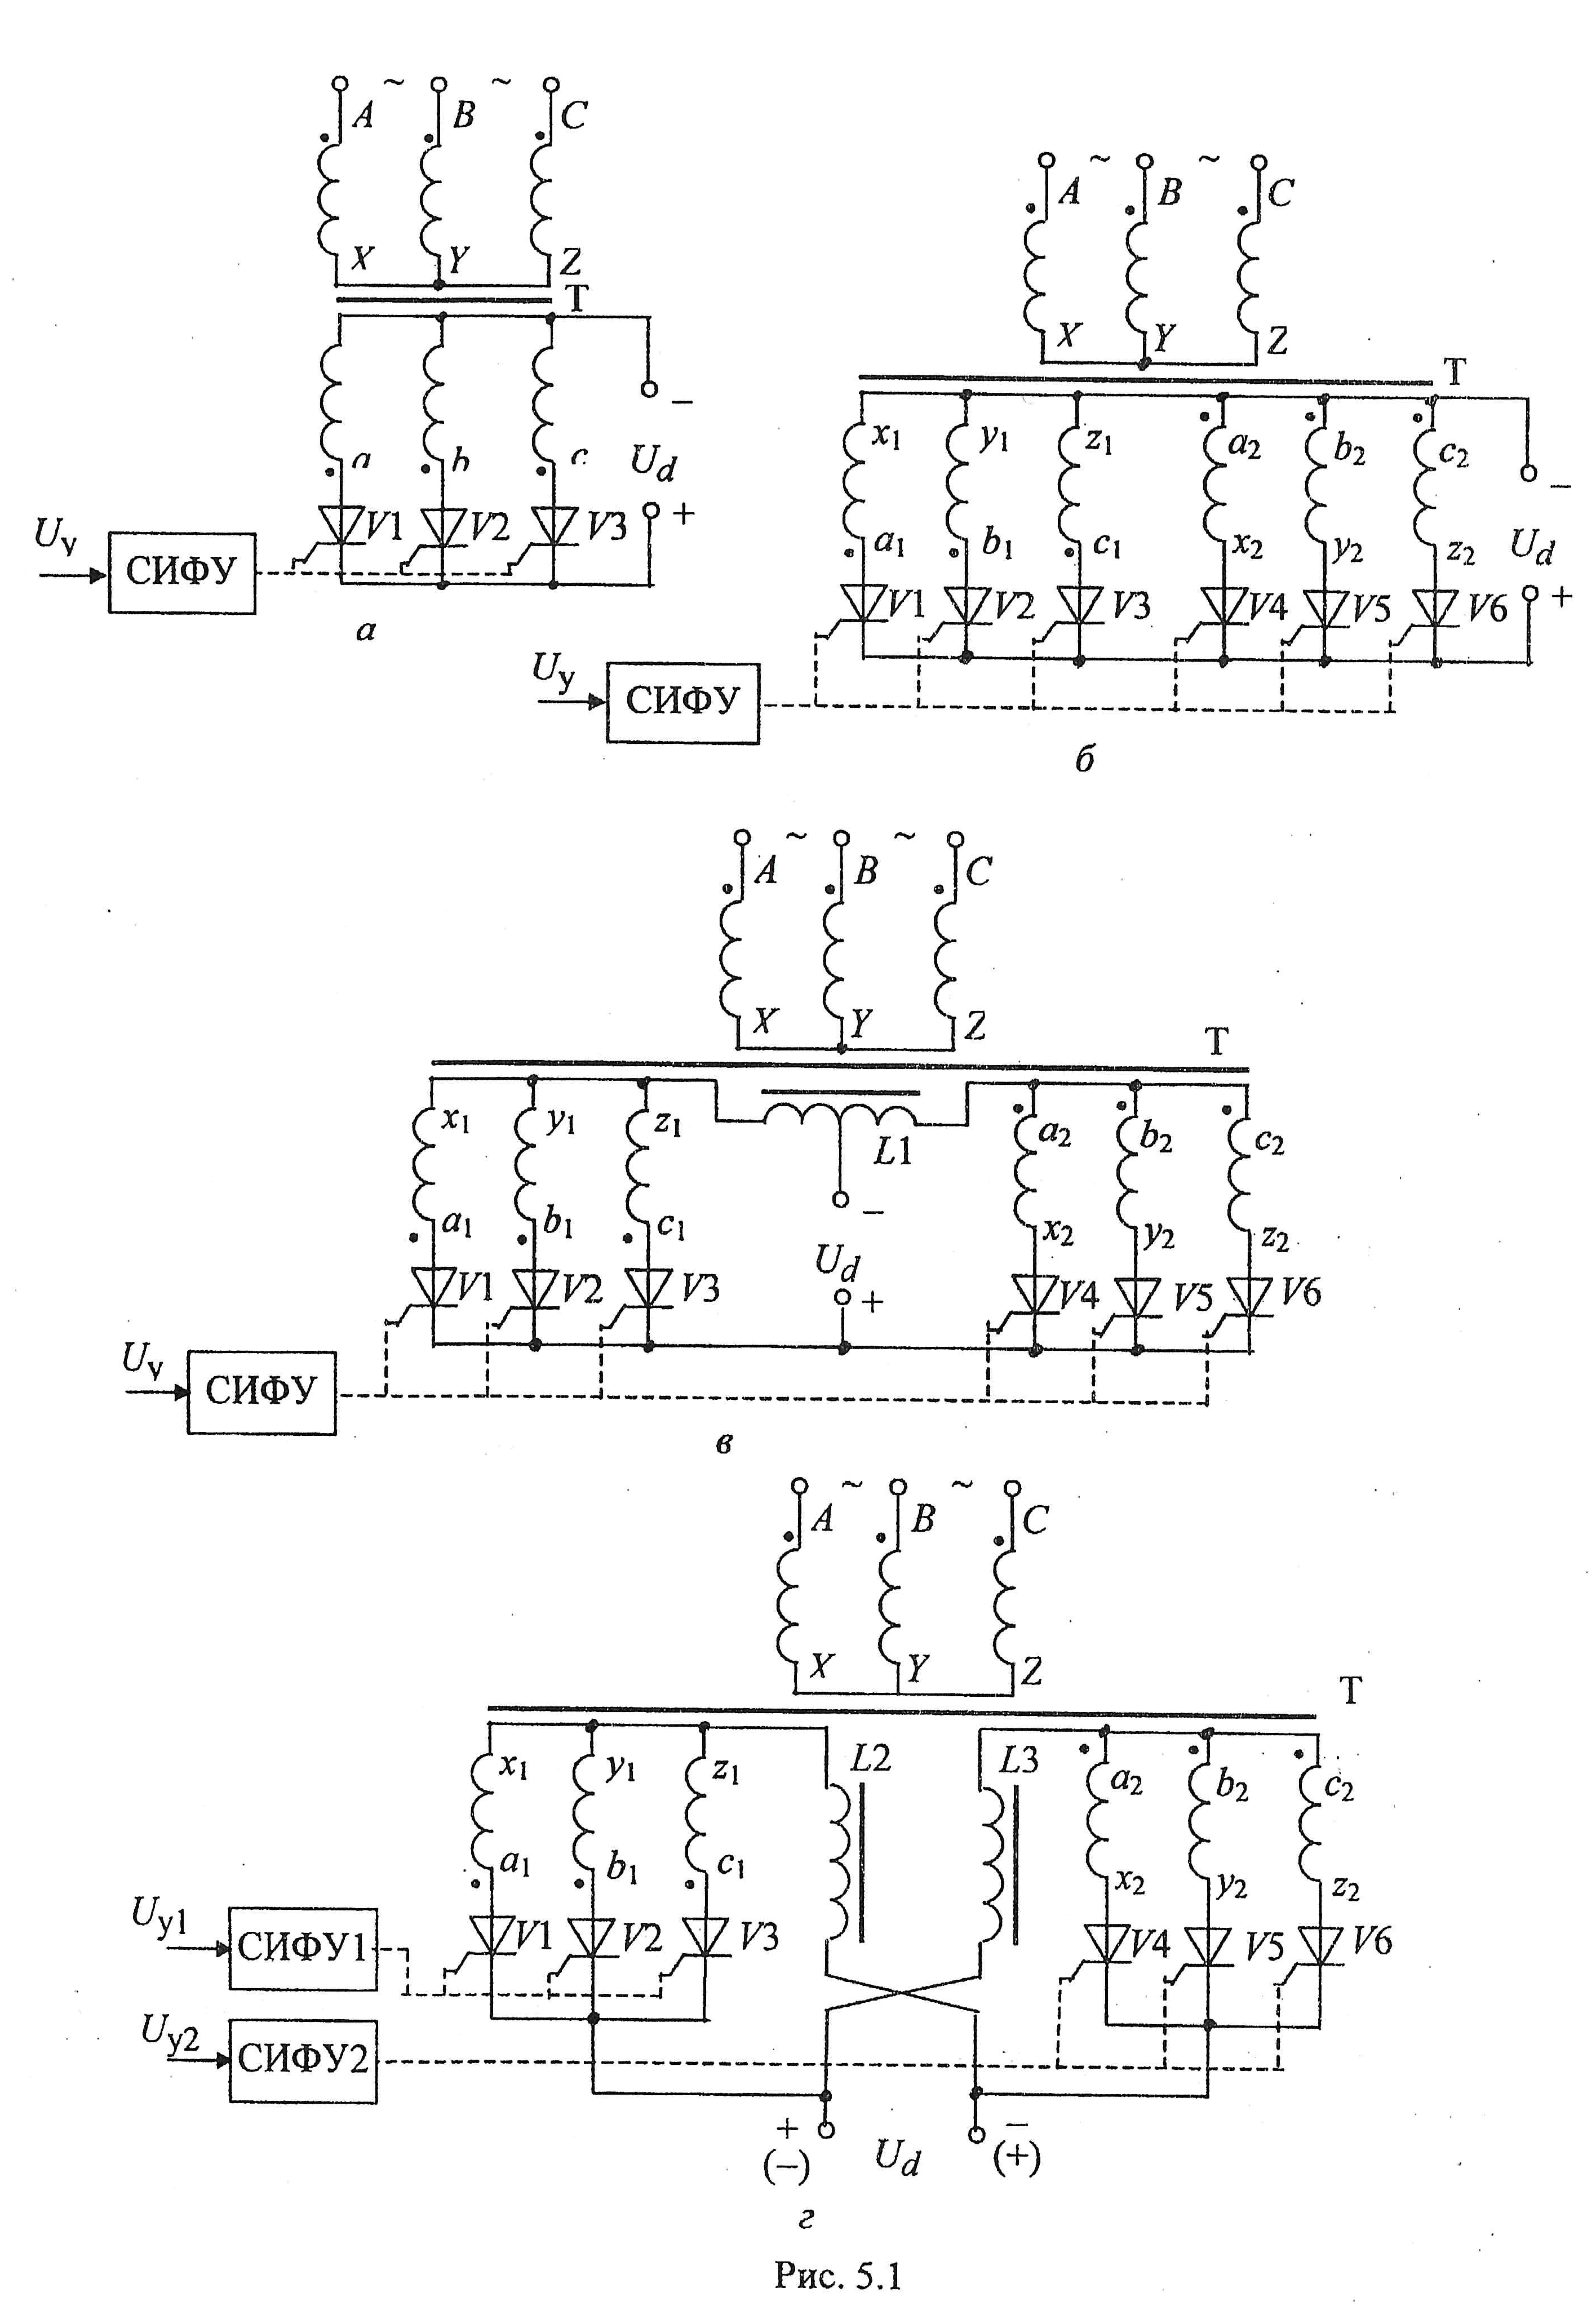
\includegraphics[scale=0.7]{ris51a}
%\caption{}
%\label{fig1}
%\end{figure}

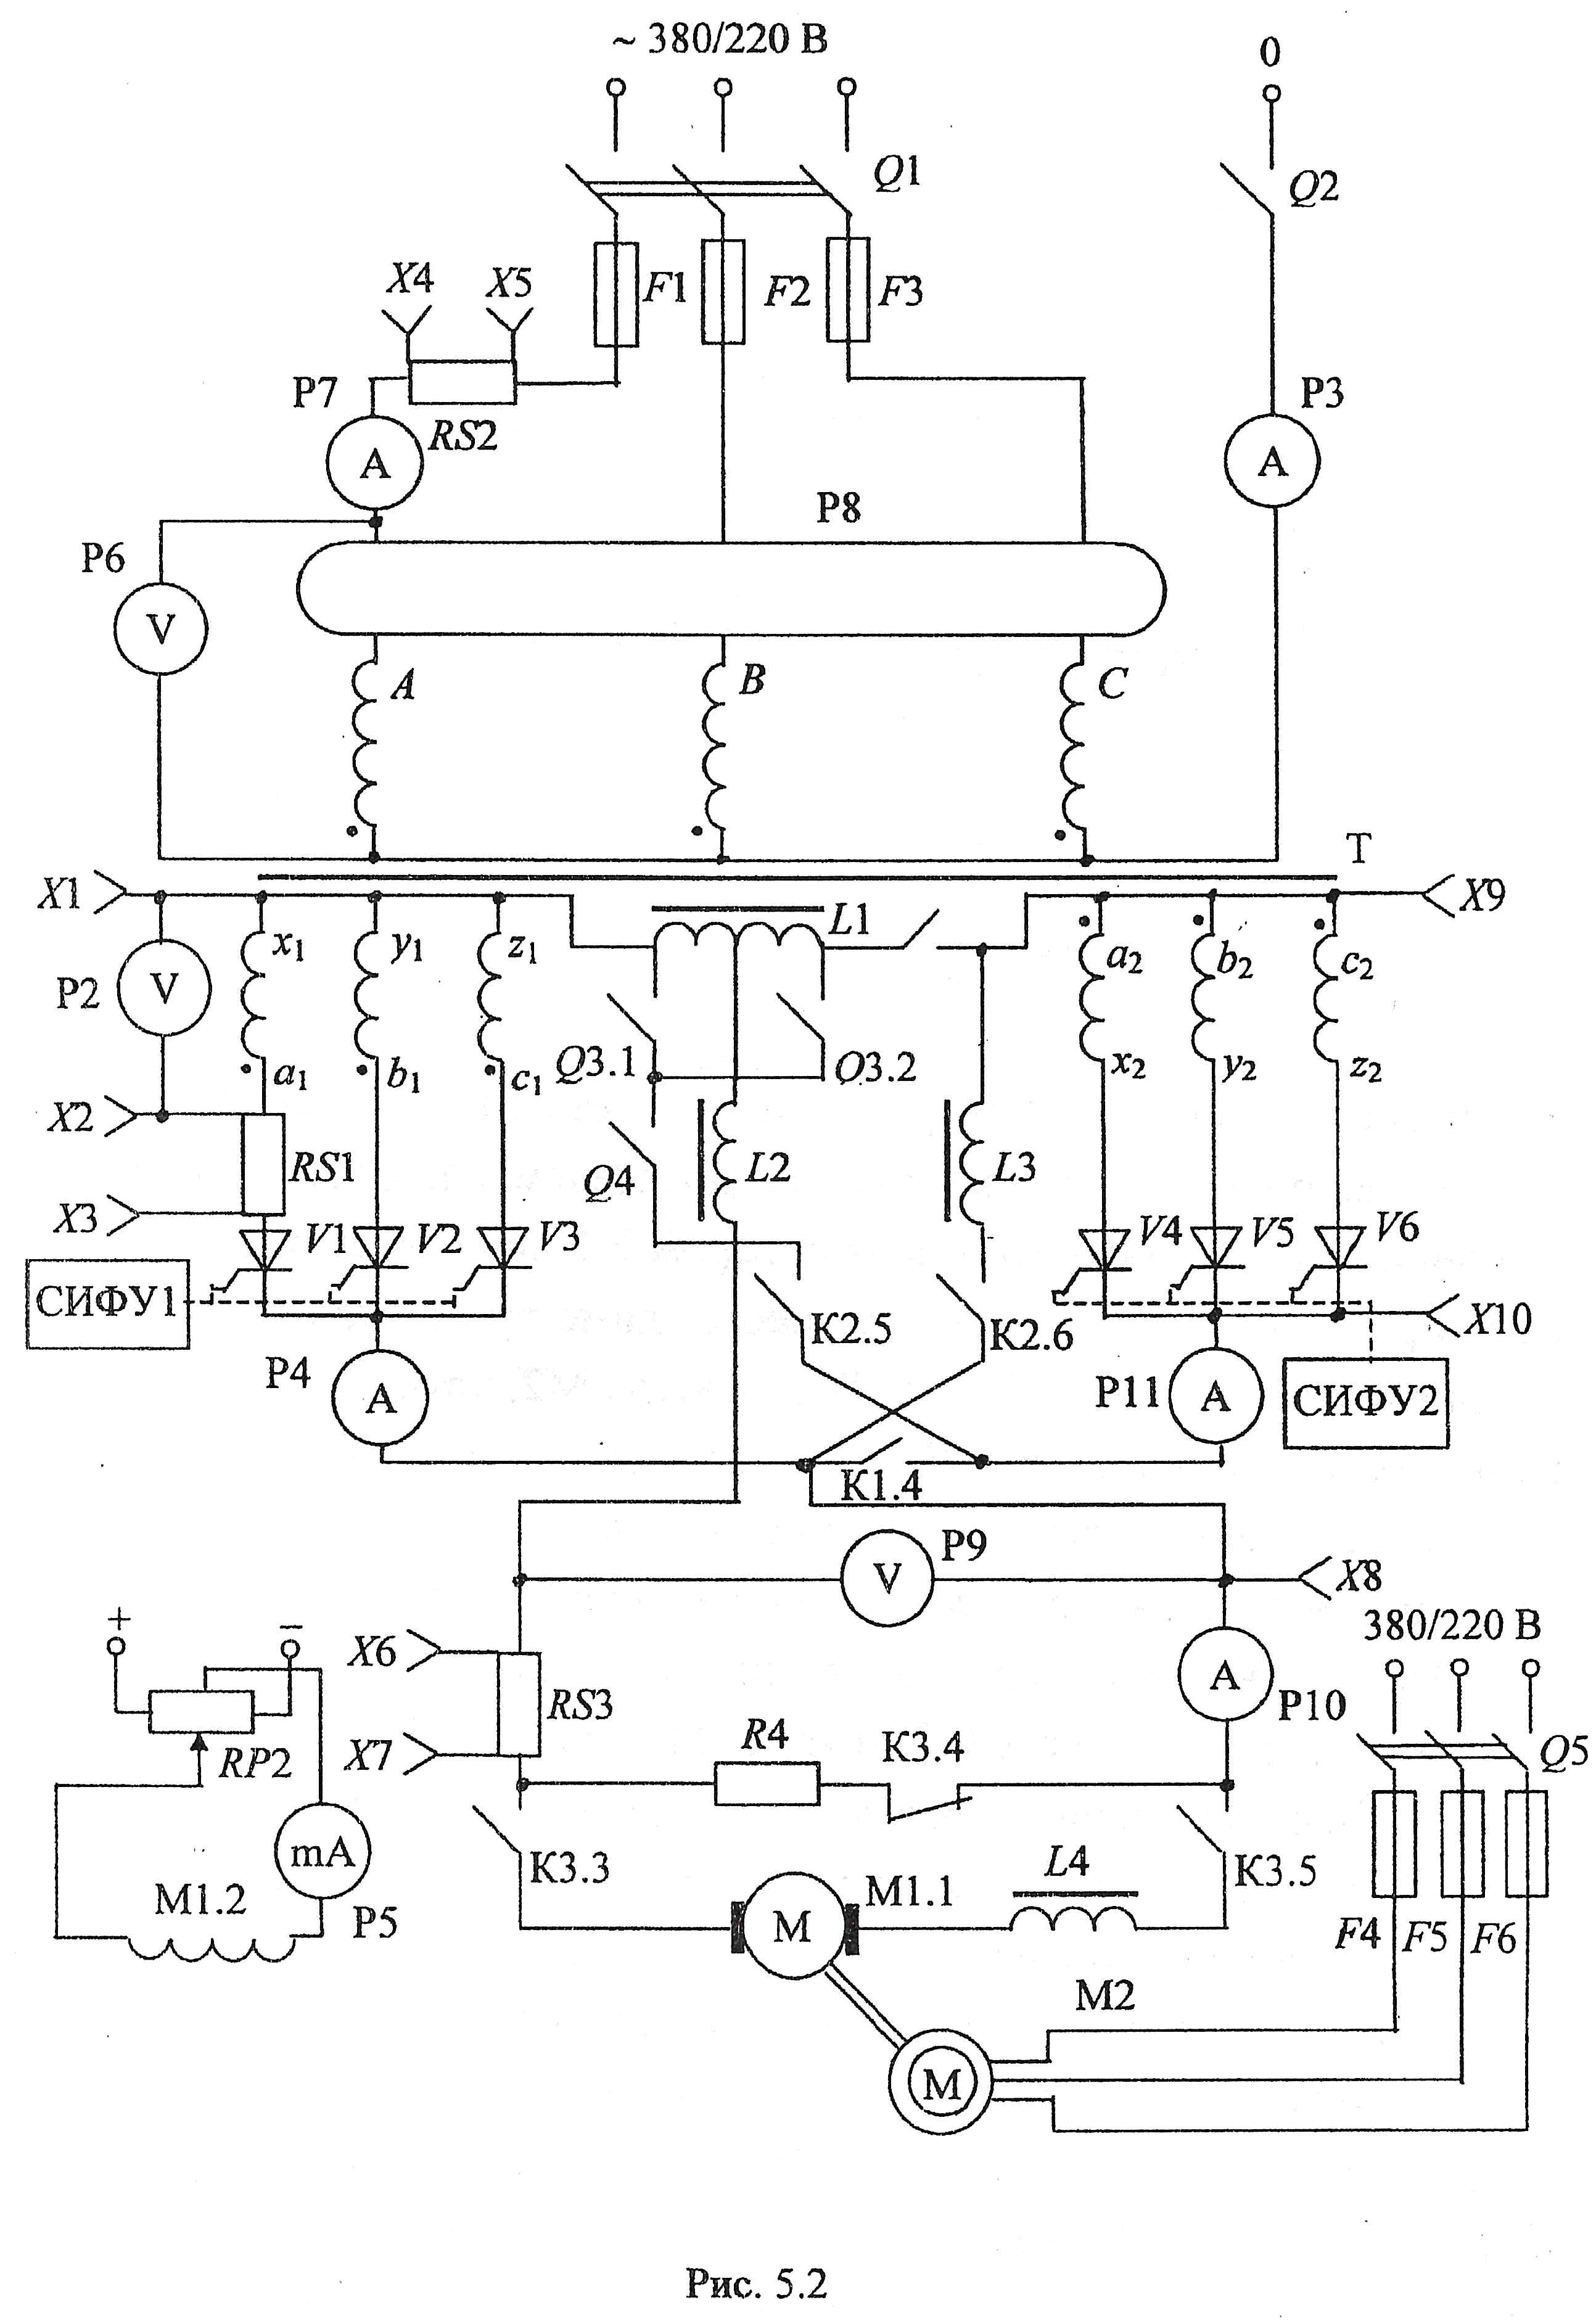
\includegraphics[scale=0.75]{ris52a}

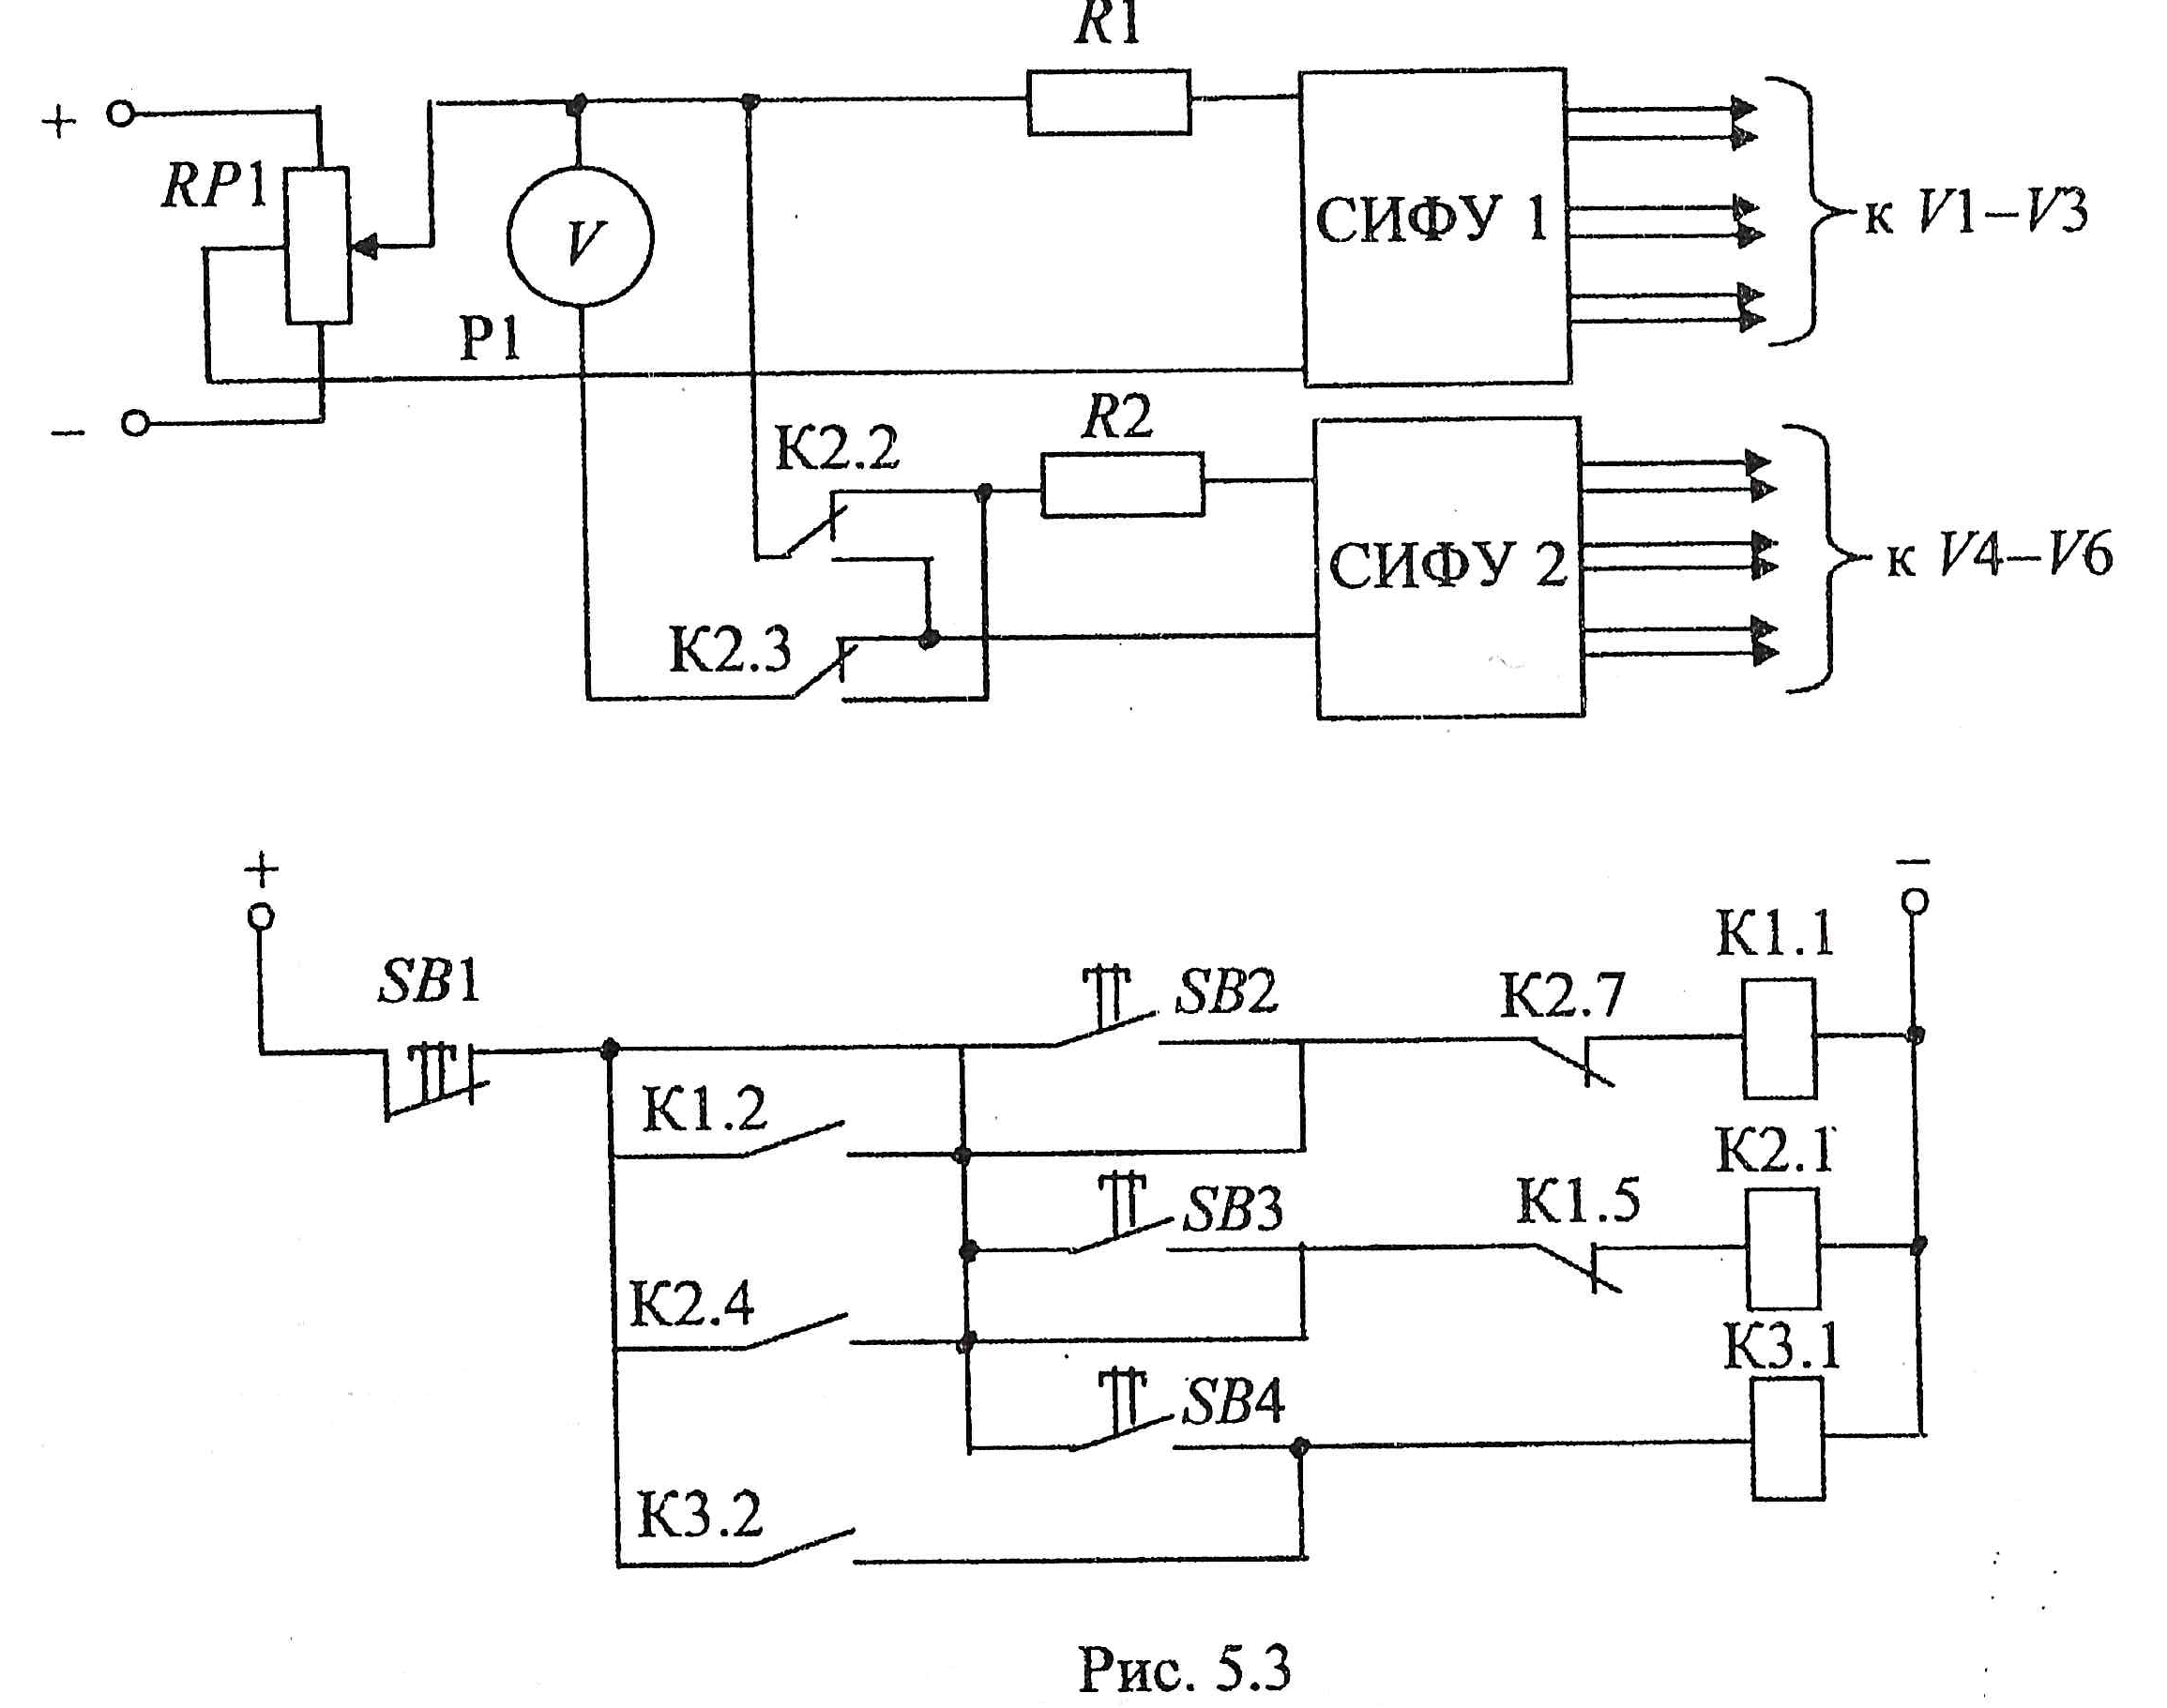
\includegraphics[scale=0.75]{ris53a}

\end{document}
